\section{Analyse der Aufgabenstellung}
\label{sec:analyse-aufgabenstellung}

Die Aufgabenstellung (siehe \appref{app:projektauftrag}) beschreibt die Rahmenbedingungen (Versuchsaufbau, Punktevergabe) des Wettbewerbs, an dem \textit{Silisloth} im Sommer 2018 teilnehmen soll. Durch eine ausführliche Analyse der einzelnen Anforderungen, die zu Beginn des Semesters vorgenommen wurde, konnte daraus ein Pflichtenheft abgeleitet werden.

\subsection{Pflichtenheft}

Das Pflichtenheft beschreibt, \textit{was} das zu erstellende System können muss, nicht \textit{wie} oder \textit{womit} dies zu bewerkstelligen ist. Deshalb wurde das Pflichtenheft als verbale Wortkette formuliert, da diese Form kein Subjekt beinhaltet, und somit noch keine Annahmen über die Lösungskomponente enthält. Das Pflichtenheft umfasst folgende Punkte:

\begin{multicols}{2}
\begin{itemize}[leftmargin=*]
\setlength\itemsep{0.2em}
\item das Startsignal erkennen
\item sich an einem Seil fortbewegen
\item die Last erkennen
\item die Last aufnehmen
\item die Last heben und senken
\item das Zielfeld erkennen
\item den Zielmast erkennen
\item die Lastkoordinaten erfassen
\item die Lastkoordinaten übertragen
\item die Lastkoordinaten anzeigen
\end{itemize}
\end{multicols}

\subsection{Funktionale Zerlegung}

Nachdem geklärt wurde, was das System leisten soll, wurde abgeklärt, durch welche Komponenten, also \textit{womit}, die jeweilige Teilaufgabe gelöst werden soll. Diese Komponenten wurden zunächst abstrakt formuliert, da die Recherche und Evaluation der tatsächlichen Lösungskomponenten erst in einer späteren Phase erfolgten. Die funktionale Zerlegung wurde eins zu eins anhand des Pflichtenheftes vorgenommen, indem den einzelnen Anforderungen ein Subjekt zugeordnet wurde:

\begin{multicols}{2}
\begin{itemize}[leftmargin=*]
\setlength\itemsep{0.2em}
\item \textit{die Startsignalerkennung} erkennt das Startsignal
\item \textit{der Fortbewegungsmechanismus} bewegt [\textit{Silisloth}] an einem Seil fort
\item \textit{die Lasterkennung} erkennt die Last
\item \textit{die Lastaufnahme} nimmt die Last auf
\item \textit{die Zielfelderkennung} erkennt das Ziel
\item \textit{die Zielmasterkennung} erkennt den Zielmast
\item \textit{die Lastkoordinatenerfassung} erfasst die Lastkoordinaten
\item \textit{die Lastkoordinatenübertraung} überträgt die Lastkoordinaten
\item \textit{die Lastkoordinatenvisualisierung} zeigt die Lastkoordinaten an
\end{itemize}
\end{multicols}

\subsection{Funktionales Blockschaltbild}
Zu den damit gefundenen (abstrakten) Lösungskomponenten wurde eine Recherche (siehe \appref{app:recherche}) durchgeführt. Aufgrund dieser Recherche konnten diese Lösungskomponenten konkretisiert und teils weiter aufgeteilt werden. Auch sekundäre Anforderungen (Stromversorgung) wurden dabei berücksichtigt. Es wurden folgende konkrete Lösungskomponenten ermittelt:

\begin{multicols}{2}
\begin{itemize}[leftmargin=*]
\item Startisgnal
\item Fortbewegung am Seil
\item Motor zur Fortbewegung
\item Lasterkennung
\item Lastaufnahme
\item Lastmotor
\item Last heben/senken
\item Zielfelderkennung
\item Stromversorgung
\item Zielmasterkennung
\item Lastkoordinatenerfassung
\item Lastkoordinatenübertragung
\item Visualisierung der Koordinaten
\end{itemize}
\end{multicols}

Weiter wurde ermittelt, welche Komponenten miteinander interagieren oder sich gegenseitig beeinflussen. Aufgrund dieser Analyse konnte ein funktionales Blockschaltbild (\imgref{fig:blockschaltbild}) erarbeitet werden, wobei die einzelnen Lösungskomponenten die Knoten und die Schnittstellen dazwischen die Kanten repräsentieren.

\begin{figure}
    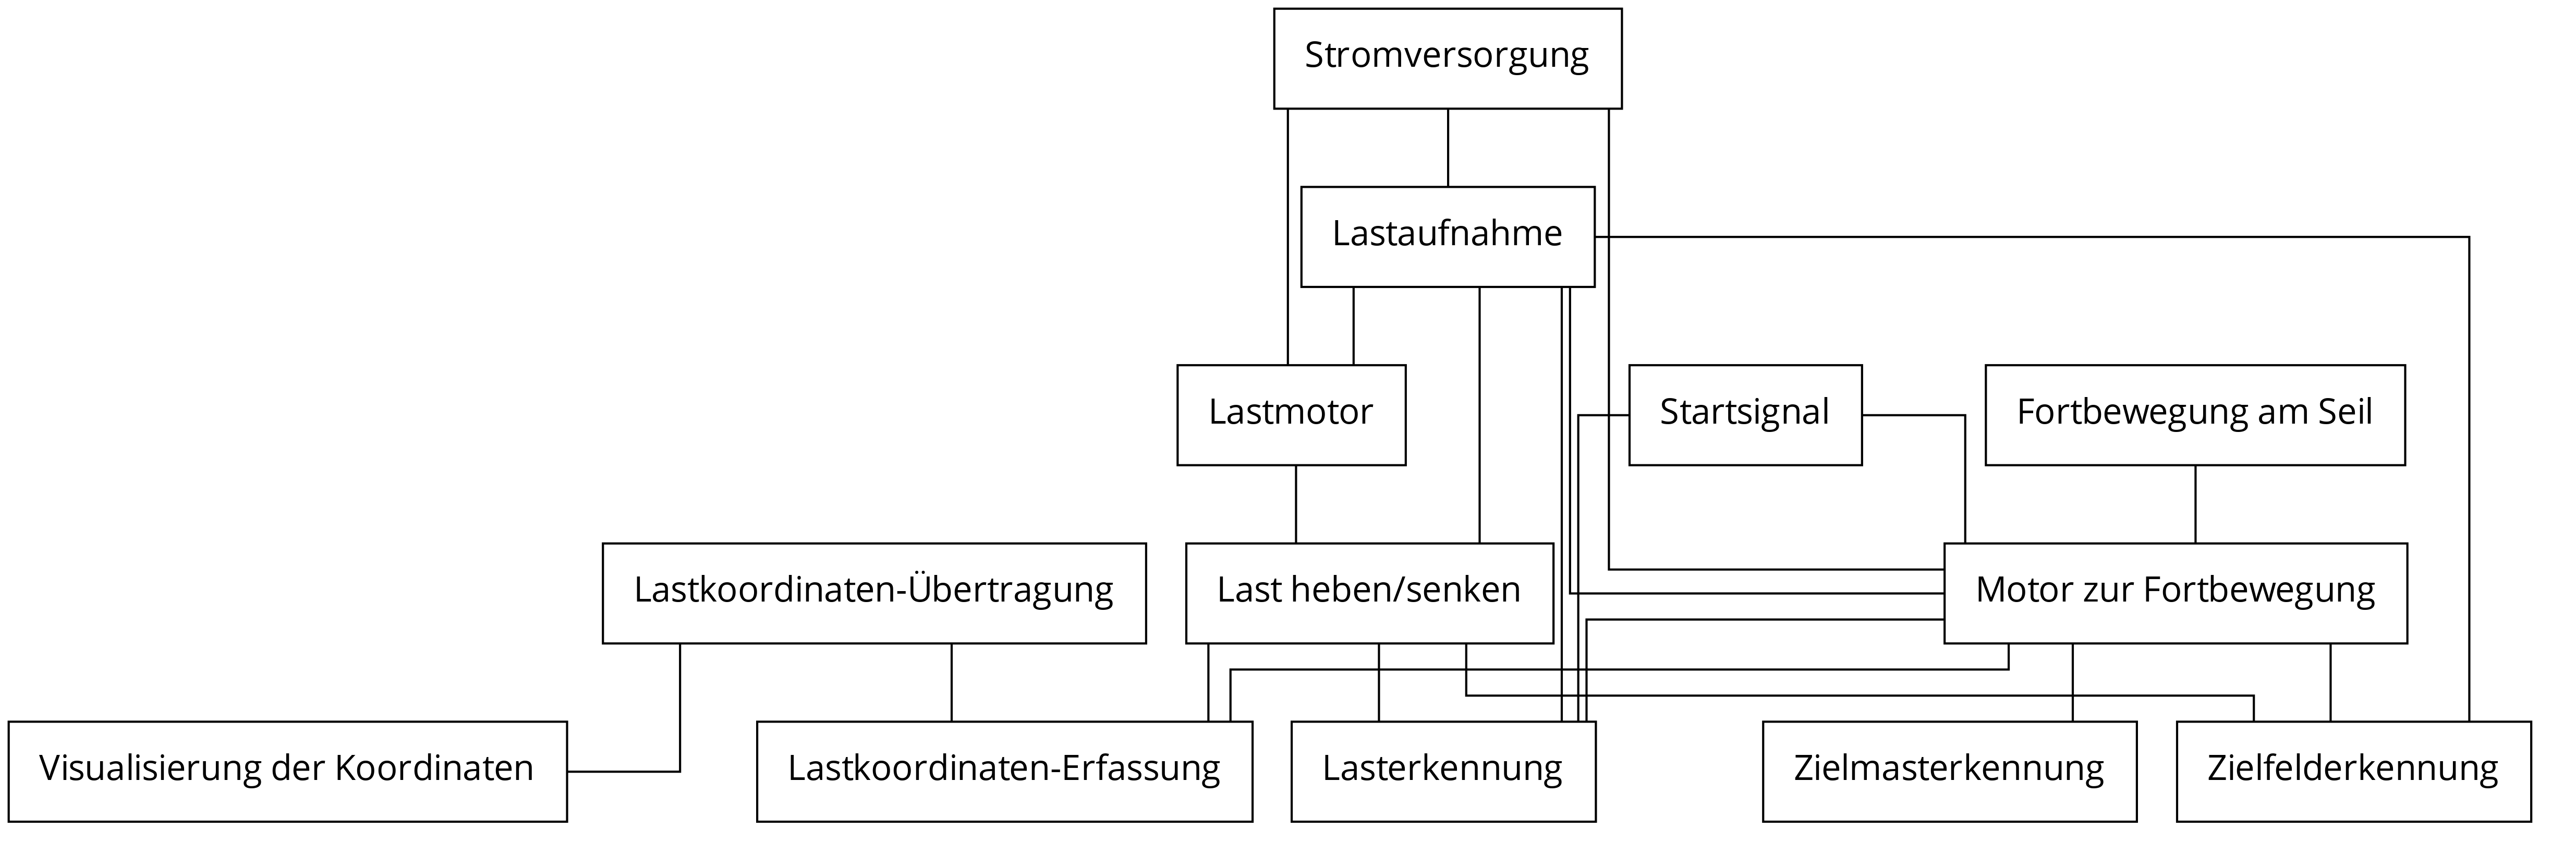
\includegraphics[width=\linewidth]{graphs/blockschaltbild.png}
    \caption{Funktionales Blockschaltbild}
    \label{fig:blockschaltbild}
\end{figure}

Zu den einzelnen Lösungskomponenten wurden mögliche Lösungsvarianten gesucht, wobei die Recherche (siehe \appref{app:recherche}) als Grundlage diente. Die dabei gefundenen Lösungsvarianten wurden in einem morphologischen Kasten gesammelt. In einer Gruppensitzung wurden mit Hilfe dieses morphologischen Kastens die einzelnen Komponenten zu Konzeptvarianten kombiniert. Zu diesem Zweck wurden vorher sogenannte Leitkriterien definiert, die vorgaben, nach welchem Kriterium die einzelnen Komponenten für ein Konzept ausgewählt werden sollten, beispielsweise «günstigste Lösung», «technisch anspruchsvollste Lösung»  (siehe \appref{app:konzeptvarianten}).

Weiter wurde eine Kompromissvariante ausgearbeitet, die zwar auch technisch anspruchsvoll und originell sein sollte, jedoch einige problematische Lösungsansätze vermied. Diese Kompromissvariante schnitt in der Nutzwertanalyse am besten ab. Eine grobe Aufwandsschätzung ergab, dass diese Kompromissvariante für die verfügbaren Gesamtressourcen der Gruppe einerseits und für die Ressourcenverteilung auf die verschiedenen Fachbereiche verteilt andererseits am ehesten erfolgreich umgesetzt werden könnte. Diese Variante -- fortan als \textit{Silisloth} bezeichnet -- wird im Weiteren genauer erläutert.

\subsection{Zeitlicher Ablauf}

\imgrefplain{fig:zeitlicher-ablauf} stellt den zeitlichen Ablauf dar. Zum Zeitpunkt \textit{Start} ist \textit{Silisloth} bereits in seine Ausgangsposition gebracht worden.

\begin{figure}
    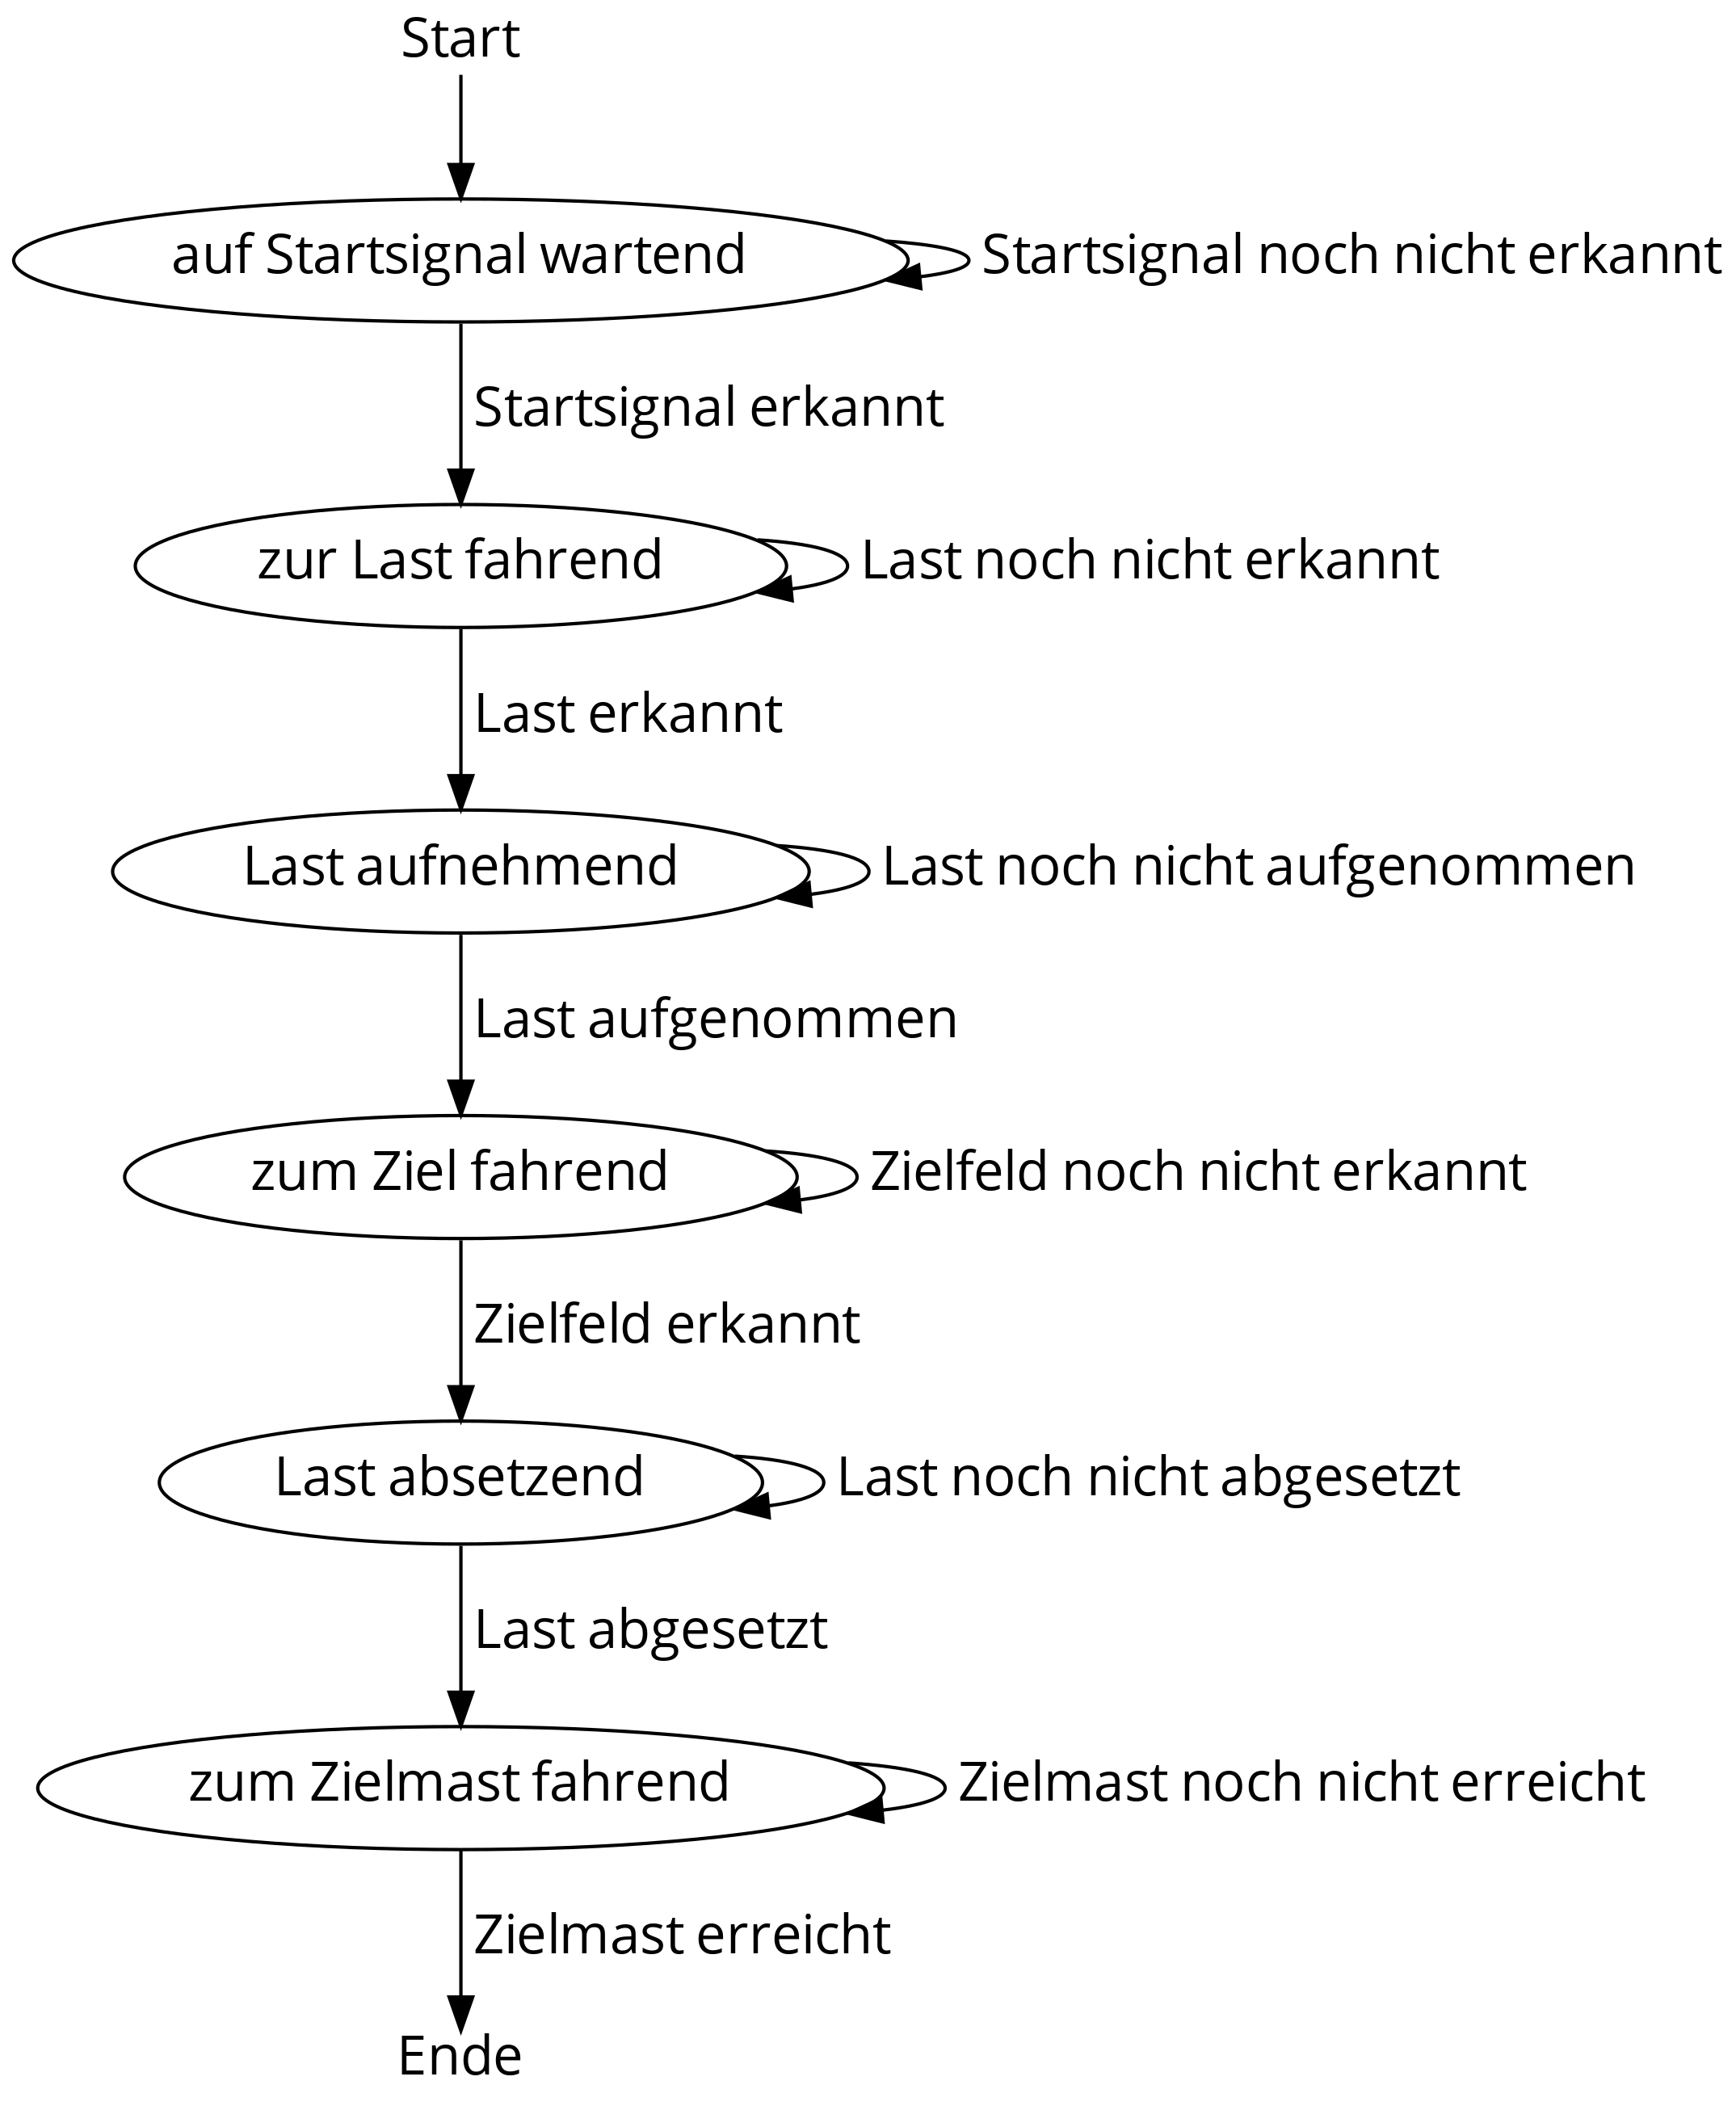
\includegraphics[width=\linewidth]{graphs/status.png}
    \caption{Der zeitliche Ablauf als Zustandsdiagramm}
    \label{fig:zeitlicher-ablauf}
\end{figure}

\begin{enumerate}
    \item \textit{Silisloth} erwartet das Startsignal. Dies wird durch den Schiedsrichter erteilt. Sobald dies erfolgt ist, wird die Starttaste betätigt.
    \item \textit{Silisloth} fährt nun los und nähert sich der Last. Das Tempo bleibt konstant, solange die Last noch nicht erkannt worden ist.
    \item Wurde die Last erkannt, kann diese aufgenommen werden. Dazu muss diese gegriffen und angehoben werden. Die Bewegung wird erst fortgesetzt, sobald die Last soweit wie möglich angehoben wurde, um keine unnötigen Schwingungen beim Anfahren zu erzeugen.
    \item Die Last wird nun über die Hindernisse hinweg in Richtung Endmast zum Ziel transportiert. Sobald das Ziel erkannt wird, kann der Abstand zum Zielfeld berechnet werden. Befindet sich \textit{Silisloth} exakt über dem Zielfeld, wird die Bewegung gestoppt und die Last abgesetzt.
    \item \textit{Silisloth} kann nun zum Ziel fahren. Die Greifapparatur muss dazu nicht erneut angehoben werden. Sobald \textit{Silisloth} den Endmast berührt, kann die Bewegung gestoppt werden. Der Ablauf ist nun zu Ende.
\end{enumerate}

